\chapter{Struttura del Magic Mirror}\label{capitolo3}
In questo capitolo verrà spiegata la struttura generale del MagicMirror, come funziona e di come veengono implementati i
moduli e il sistema di messaggistica.
Il Magic Mirror \`e un progetto ideato e sviluppato da Michael Teeuw, successivamente esteso nelle sue funzionalit\`a da una moltitudine di utenti su GitHub.
Una prima versione \`e stata scritta completamente in Python, mentre successivamente \`e stata creata una seconda versione nella quale si \`e preferito l'utilizzo di Electron,
che ha comportato una variazione di linguaggio, a favore di Javascript. In questo modo \`e stato possibile implementare un'interfaccia esteticamente pi\`u gradevole
e API pi\`u intuitive.
L'idea dell'autore \`e nata rifacendosi allo specchio magico dell'omonima fiaba
scritta dai fratelli Grimm, Biancaneve e i Sette Nani.\\
Il software viene mostrato attraverso un
comune monitor, trasmettendo immagini poste su uno sfondo completamente nero. Applicando sopra
una semplice pellicola a specchio (la quale da un lato permette di specchiarsi e dall'altro di vedere
attraverso) si crea un effetto particolare per cui una persona riesce a specchiarsi
e allo stesso tempo riesce a vedere le scritte o le immagini trasmesse dal monitor,
come mostrato in figura \ref{fig:MM}.
\\[2\baselineskip]
\begin{figure}[H]
    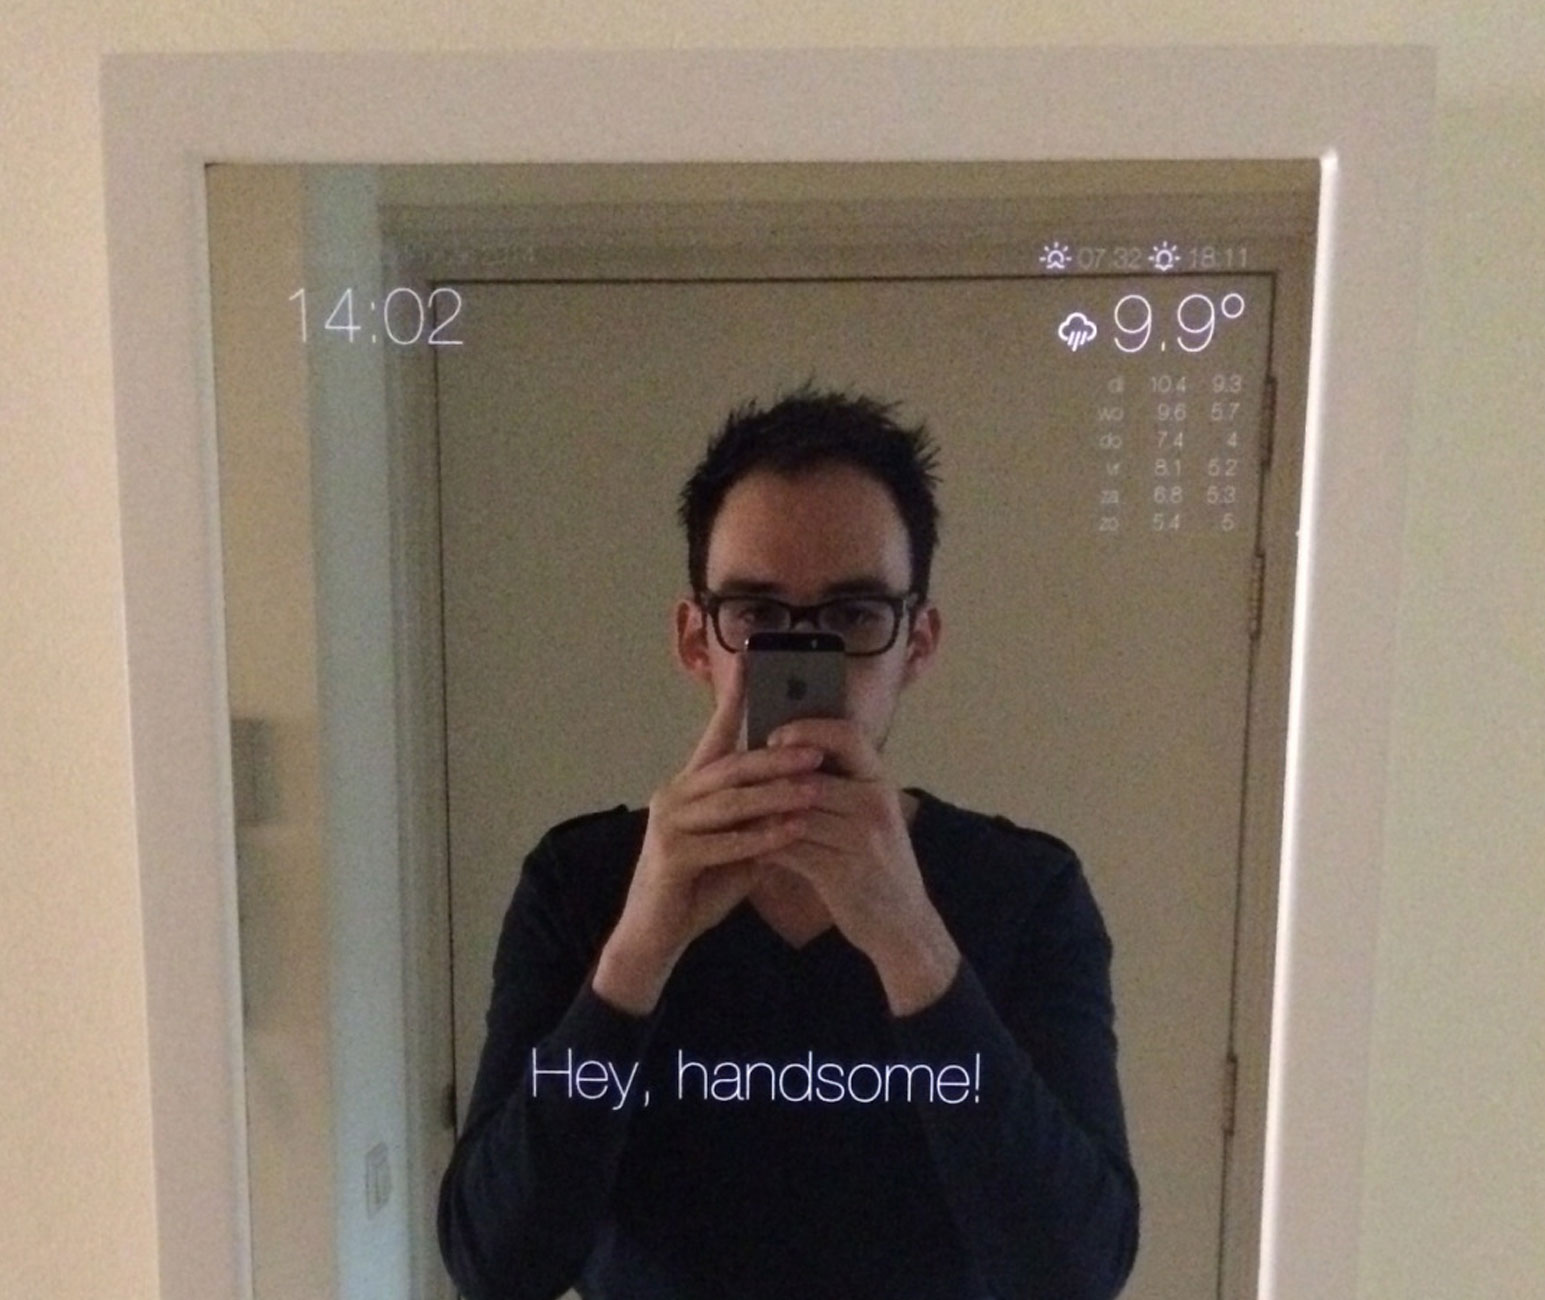
\includegraphics[width=1\textwidth, height=0.6\textheight]{magic_mirror}
    \caption{Magic Mirror by Michael Teeuw}
    \label{fig:MM}
\end{figure}

\section{Il MM dall'alto livello}\label{cap:MMalto}
Il MM è una applicazione con diverse API e strutture che permettono l'interazione e la comunicazione tra i moduli.
Si possono individuare alcuni elementi principali rappresentati in figura \ref{fig:struttMM}:
\begin{figure}[H]
    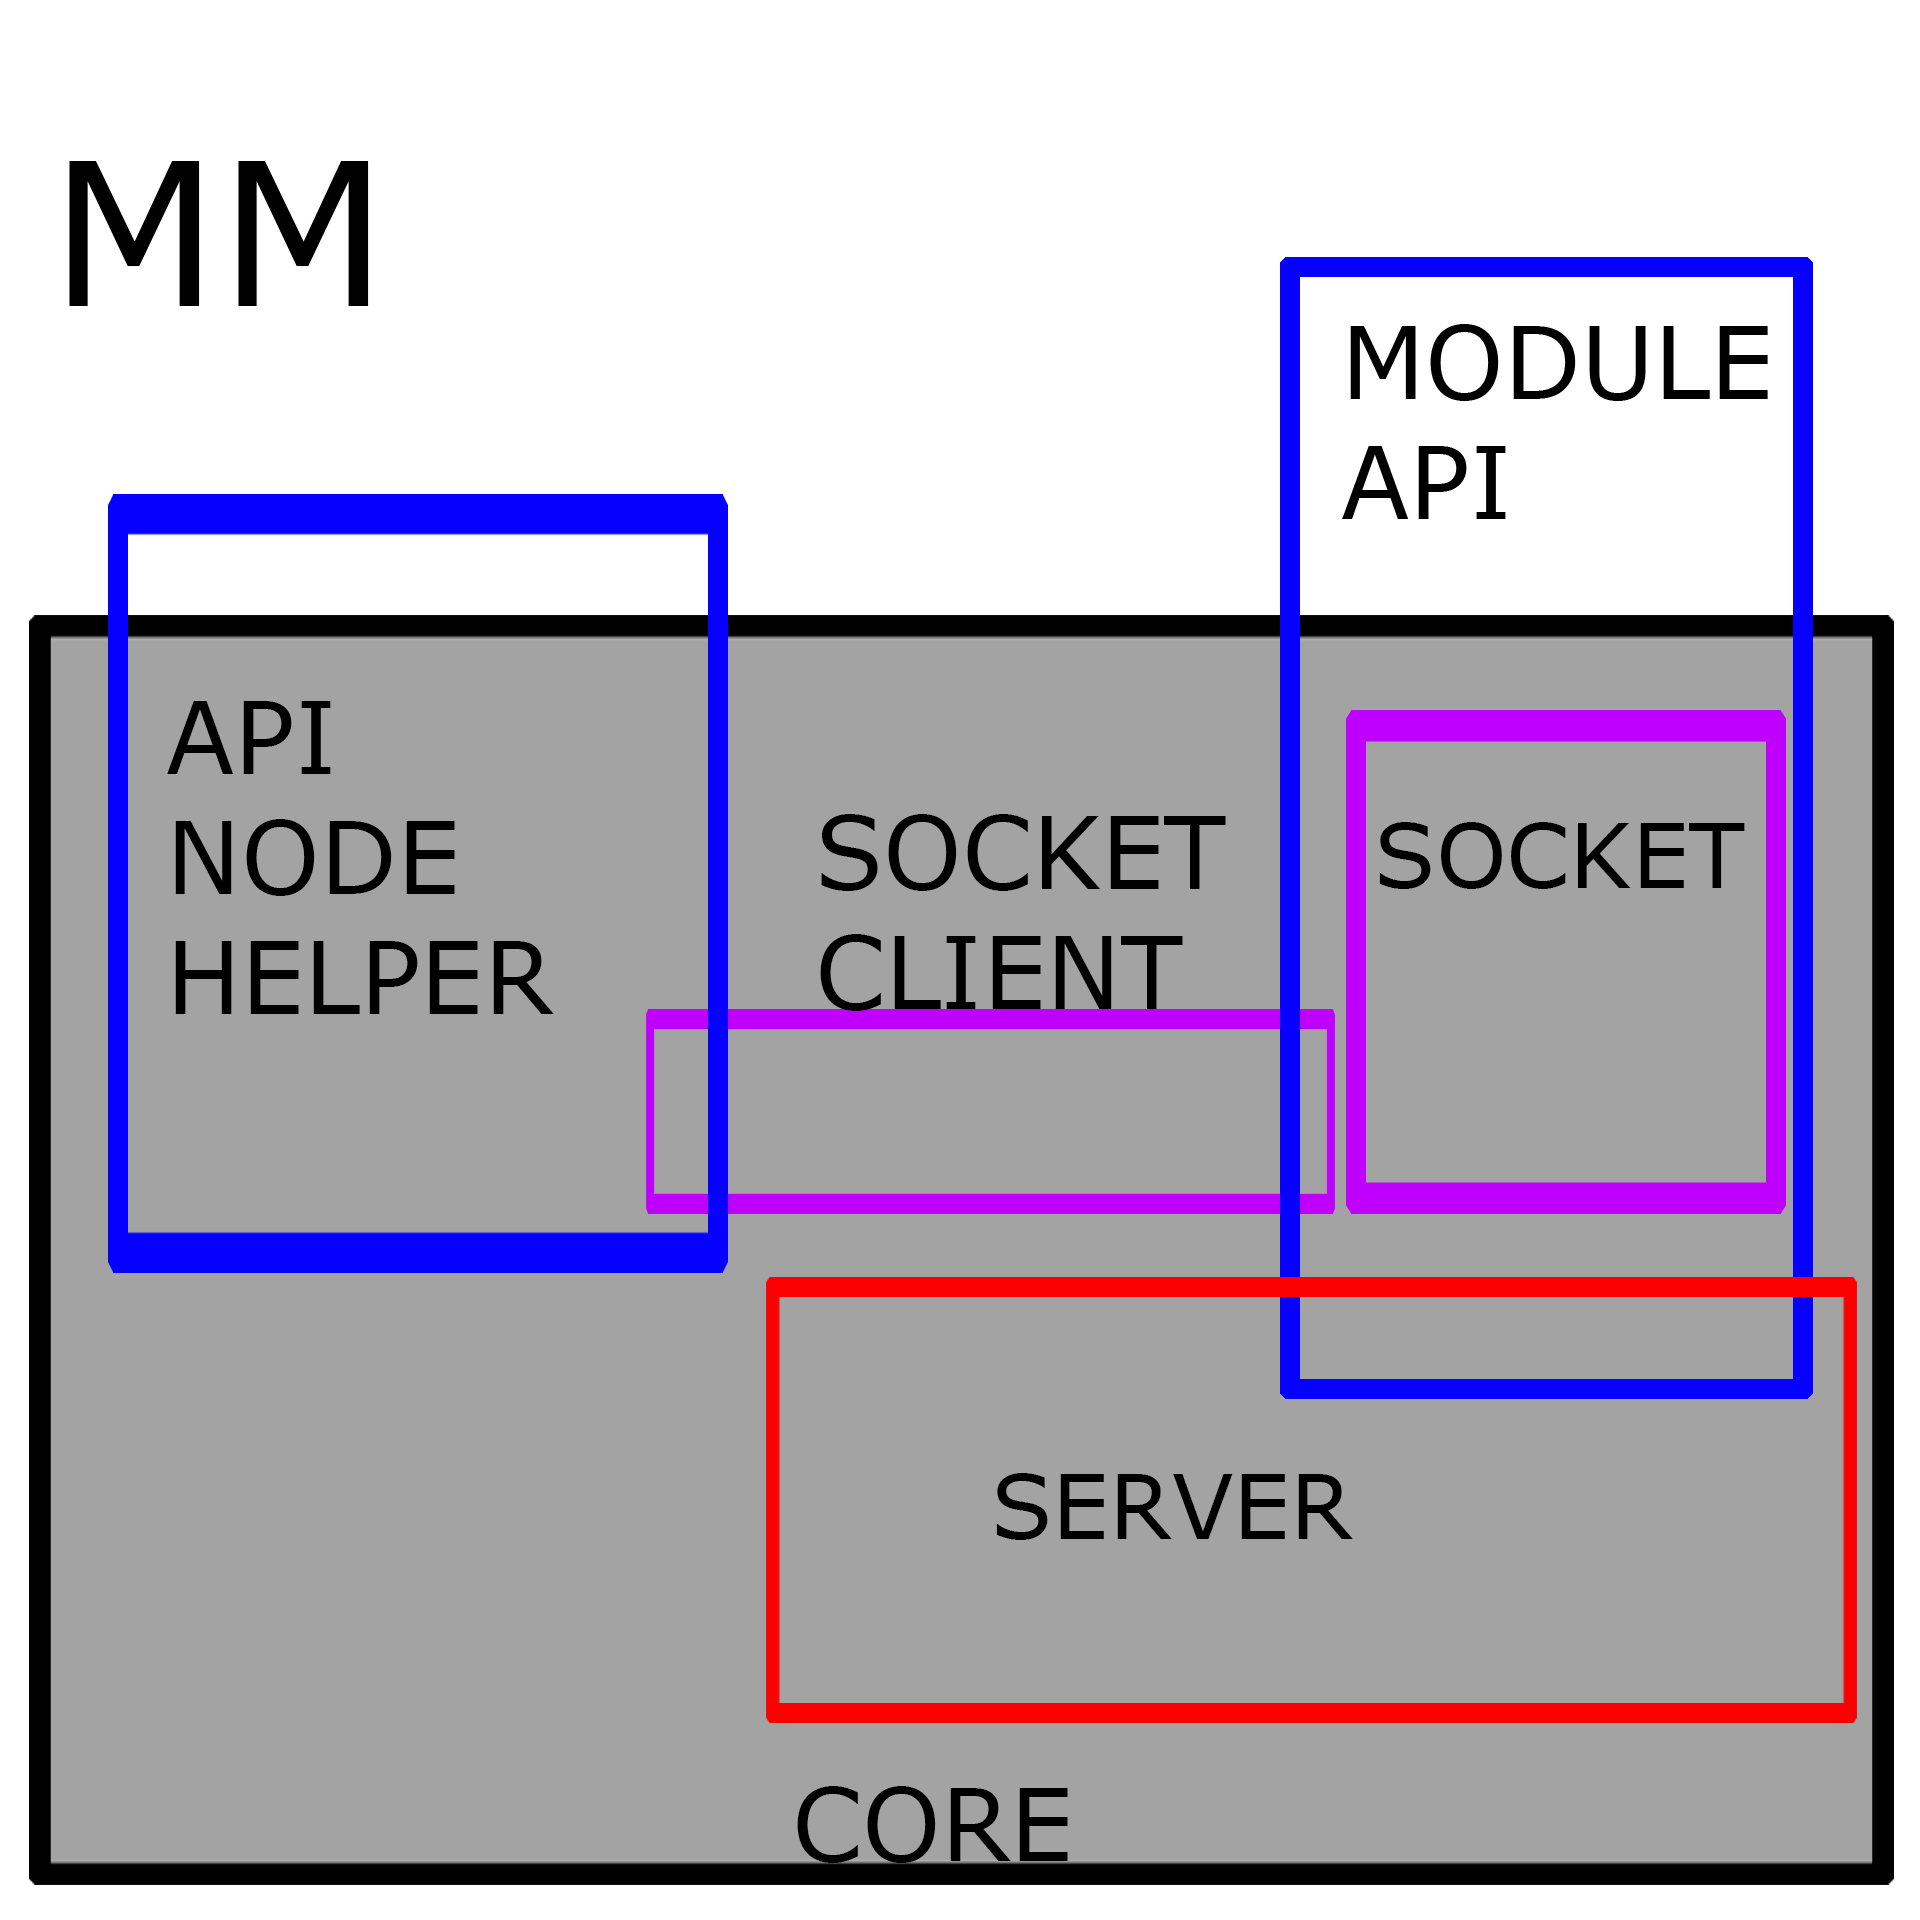
\includegraphics[width=1\textwidth, height=0.6\textheight]{struttMM}
    \caption{Struttura MagicMirror}
    \label{fig:struttMM}
\end{figure}
\begin{itemize}
\item Il core, il cuore del MM dove gira il codice principale.
\item Il server, che gira in locale, usato per restituire la pagina html con i dati al browser di Electron
\item Le API per i moduli, i metodi e funzionalità esposti dla MM per poter itegrare i moduli creati
\item Le API per i Node Helper, i metodi e funzionalità esposti dla MM per poter itegrare i NodeHelper
dei relativi moduli
\item Il Socket, entità che si trova in mezzo alle API e ne fornisce un canale di comunicazione
\item Il SocketClient, entità che si trova tra le API delle applicazioni e dei Node Helper, e fornisce il canale
di comunicazione tra questi due\\[2\baselineskip]
\end{itemize}

\section{Avvio ed Escuzione}
Il Magic Mirror viene avviato tramite linea di comando, la quale esegue
il codice di un file Javascript, il cui percorso viene indicato nel documento \textit{package.json}, descritto nella sezione \ref{cap:Electron}.
Il file contiene il codice di Electron, che si occupa della creazione di una nuova finestra browser, il cui compito
è di mostrare l'output dei moduli del MM, e l'avvio del codice che rappresenta il core, che carica tutte le strutture princiapli del MM.
La pagina costruita e l'output dei moduli sono un insieme di Document Object Model (DOM), ovvero oggetti HTML che compongo una pagina web, che vengono mostrati solo dopo l'avvio di tutti i moduli attivi.
Le strutture principali caricate dal MM sono le seguenti:
\begin{itemize}
\item gli end-point delle API per le applicazioni, che sono le interfacce usate per leggere e caricare le applicazioni inserite nel Magic Mirror.
\item gli end-point delle API per i Node Helper, per la gestione dei questi ultimi. Sono strutture opzionali usate per collegamenti
esterni al Magic Mirror (per esempio, con API di un servizio cloud). Ogni applicazione ha il proprio Node Helper con cui pu\`o comunicare tramite messaggi in modo
simile a come comunicano le applicazioni tra di loro.
\item un "Socket" e un "Socket-Client", entit\`a principali che definiscono le funzioni per lo scambio dei messaggi tra le applicazioni e i rispettivi Node Helper.
\item un Logger, implementato per tenere i log dell'applicazione e degli evenutali errori. Usato pricipalmente per il debugging.
\item un file di configurazione, nel quale sono specificati il nome e le coordinate per la posizione dei vari moduli
all'interno della pagina.\\[2\baselineskip]
\end{itemize}
Inoltre viene inizializzato un server, il cui compito \`e quello di trasmettere la pagina resa, con gli output delle varie applicazioni,
al browser precedentemente avviato.

\subsection{Il file di Configurazione}\label{cap:MMconf}
Come discusso nella sezione \ref{cap:Config}, il Magic Mirror carica un file di configurazione, che è composto dai seguenti campi:
\begin{itemize}
\item la porta del server
\item una whitelist, ovvero un IP oppure un range di IP che possono collegarsi allo specchio
\item la lingua principale del sistema
\item il formato dell'ora (12h o 24h)
\item unit\`a di misura usata (ad esempio, metrica), usata per gestire la distanza dei DOM
\item una lista di applicazioni (in formato JSON) da caricare con la relativa posizione nella pagina. Per ogni applicazione deve necessariamente comparire il
nome e la posizione; opzionalmente si possono inserire un campo  \textit{header} e un campo \textit{config} specifico per l'applicazione, come mostrato
nell'esempio in figura \ref{code:configapp}.
\begin{lstlisting}[label={code:configapp}]
{
	"module": 'nome dell'applicazione',
	"position": 'la posizione dell'applicazione all'intenro dello specchio',
	"header": 'una stringa che viene stampata sopra all'applicazione',
	"config": { opzioni varie in formato JSON }
}
\end{lstlisting}
\end{itemize}
La lingua, il formato dell'ora e l'unit\`a di misura usata sono parametri messi a disposizione dal sistema per la creazione di un'applicazione
(ad esempio, il display di un orologio).

\section{Implementazione di un'applicazione}\label{cap:app}
La modifica del file di configurazione del Magic Mirror appena descritta serve per "notificare" la presenza delle applicazioni a quest'ultimo,
ma perch\`e possano funzionare \`e necessario che rispettino alcune specifiche regole.
Per inserire il codice dell'applicazione all'interno dello specchio \`e necessario creare una cartella con un nome identificativo dell'applicazione
nella directory \textit{Modules}.
Dentro la cartella appena creata devono essere inseriti:
\begin{itemize}
\item 1 file Javascript (JS), ovvero il documento principale con lo stesso nome della cartella appena creata. Contiene il codice dell'applicazione, il quale
conterr\`a a sua volta il codice per la creazione dei DOM
\item 1 file Cascading Style Sheets (CSS), per modificare l'estetica del DOM della relativa applicazione (opzionale)
\item 1 file node\_helper.js, che \`e il Node Helper associato alla specifica applicazione (opzionale)
\item Altri file necessari all'applicazione (immagini, JSON, etc)\\[1\baselineskip]
\end{itemize}
%Il file Javascript principale dell'applicazione viene caricato per primo dal Magic Mirror, e consiste in una chiamata di funzione con i seguenti due parametri:
%\begin{lstlisting}[language=JavaScript]
%{
%	Module.register("Nome dell'applicazione", { /* lista JSON di oggetti contenenti funzioni o variabili */});
%}
%\end{lstlisting}
%Il primo parametro \`e una stringa contenente il nome dell'applicazione: quest'ultimo deve essere necessariamente uguale al nome della cartella e al nome
%del file Javascript. Il secondo parametro, invece, \`e una lista JSON contenente funzioni o variabili (come in figura *da inserire*).
\iffalse
Le funzioni offerte dalle API sono:
\begin{itemize}
\item defaults: {}, una lista di variabili che possono essere richiamate all'interno di una qualsiasi funzione tramite il comando \textit{this.config.variabile}.
I valori di queste possono essere sovrascritti modificando il campo \textit{config} del relativo modulo nel file di configurazione del Magic Mirror.
\item start: function(){}, funzione che viene eseguita quando tutte le applicazioni dello specchio sono state caricate (ovvero quando sono stati creati tutti i relativi DOM)
\item getDom: function(){}, funzione che deve ritornare un DOM (un oggetto HTML contenente i dati da mostrare a schermo), creato tramite funzioni Javascript
\item getStyles: function() { return []}, funzione che ritorna un array di file (in formato CSS) usati per l'estetica del DOM. Possono essere nella cartella dell'applicazione
oppure ottenuti tramite link
\item getTranslations: function() {	return {en: "translations/en.json", de: "translations/de.json"}}, funzione per tradurre l'applicazione in pi\`u lingue;
se disponibile, viene caricata la traduzione in base alla lingua configurata nel software
\item getHeader: function() {	return this.data.header;}, funzione che stampa il campo \textit{header} della configurazione, con la possibilit\`a concaternarla
ad una stringa o ad un parametro
\item notificationReceived: function(notification, payload, sender) {}, funzione che serve per ricevere messaggi da altre applicazioni. Viene richiamata alla ricezione
\item socketNotificationReceived: function(notification, payload){}, funzione che serve per ricevere messaggi dal Node Helper della relativa applicazione\\[1\baselineskip]
\end{itemize}
Inoltre possono essere aggiunte delle funzioni necessarie all'applicazione implementandole con la stessa sintassi di quelle di default.
\\[1\baselineskip]
Il Node Helper, invece, viene caricato come libreria ed esportato insieme all'applicazione quando viene caricata dallo specchio. Per inizializzarlo sono
necessari i comandi:
\begin{lstlisting}[language=JavaScript]
{
  var NodeHelper = require("node_helper");
  module.exports = NodeHelper.create({/* lista JSON di oggetti contenenti funzioni*/});
}
\end{lstlisting}
A differenza del file Javascript principale, l'unica funzione messa a disposizione dall' API \`e:
\begin{lstlisting}[language=JavaScript]
{
  start: function() {}
}
\end{lstlisting}
mentre \`e possibile implementare le proprie funzioni con la stessa sintassi.
\fi
\section{Messaggistica del MM}\label{cap:MMmess}
Nella sezione \ref{cap:MMalto} \`e stato gi\`a accennato che il Magic Mirror implementa un meccanismo di messaggistica sfruttando un sistema di socket integrato,
utile per l'organizzazione e la moderazione delle applicazioni tramite l'utilizzo di funzioni messe a disposizione dall'API.
Sono presenti due classi socket:
\begin{itemize}
\item Socket, classe che fornisce le funzioni per ricevere e mandare messaggi tra i moduli del MM. Con questo socket quando la spedizione
del messaggio è in broadcast usando la funzione \textit{sendNotification(notification, payload)}. Il primo parametro è una stringa che identifica
il messaggio, il secondo parametro è opzionale ed può essere usato per inserire il corpo del messaggio.
La ricezione del messaggio viene gestita con la funzione \textit{notificationReceived(notification, payload, sender)}, i primi due parametri sono
uguali a quelli della funzione per spedire, il terzo parametro contiene il nome del
modulo che ha mandato il messaggio
\item Socket Client, classe che fornisce le funzioni per ricevere e mandare messaggi tra il modulo e il suo NodeHelper. Per spedire
i messaggi viene usata la funzione \textit{sendSocketNotification(notification, payload)}, mentre la ricezione viene gestita con la funzione
 \textit{socketNotificationReceived(notification, payload)}. I campi di queste due funzioni sono gli stessi descritti nel punto precedente.\\[1\baselineskip]
\end{itemize}
